\begin{figure}
\centering	
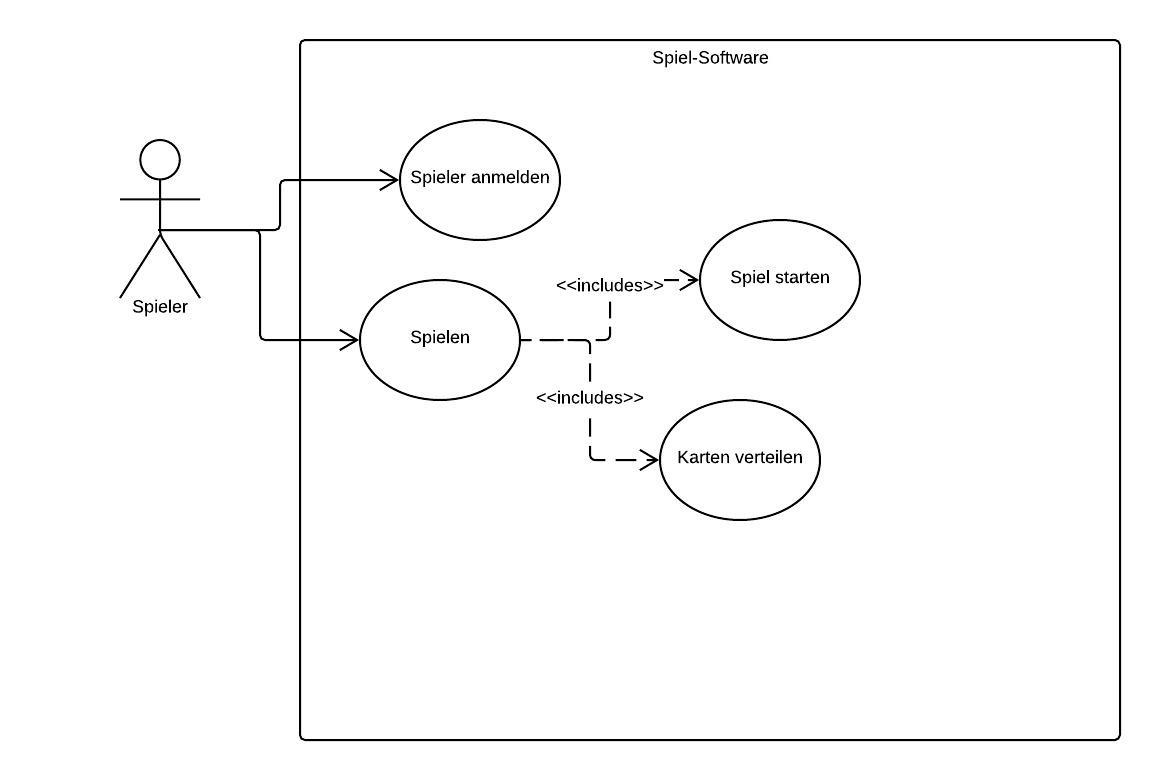
\includegraphics[width=0.9\textwidth]{img/ucd.jpg}
\label{fig:sys}
\caption{Beispiel für ein Systemgrenzendiagramm (Use Case Diagramm), das vor Abgabe anzupassen ist.}
\end{figure}

\section{Systemgrenze (Use Case Diagramm)}

Die Systemgrenze wird in der Abbildung~\ref{fig:sys} dargestellt\footnote{Weitere Erklärungen und Spezifizierungen, die sich auf Abgrenzungen der Verantwortlichkeiten vom System und weiteren Akteuren/Systemen beziehen, können hier spezifiziert werden.}. 


\section{Beschreibungen der Anwendungsfälle}

Hinweis: Alle Systemfunktionen sind mit Anwendungsfällen zu decken! (Und dieser Hinweis ist zu löschen, wie auch der Beispielfall).

\newcounter{uc}\setcounter{uc}{10}

\begin{description}[leftmargin=5em, style=sameline]

	\begin{lhp}{uc}{UC}{uc:beispiel}
		\item [Name:] Name des Use Cases\footnote{Dieser Anwendungsfall ist offensichtlich ein/e Beispiel/Anleitung und muss gelöscht werden.}.
		\item [Ziel:] Ziel und Zweck des Use Cases.
		\item [Akteure:] Akteure (auch benachbarte Systeme können Use Cases anfeuern), die den Use Case aktivieren können.
		\item [Vorbedingungen:] Eigenschaften des Systemzustands, in dem die Aktivierung des Use Cases möglich ist.
		\item [Eingabedaten:] Daten, die für die Ausführung des Use Cases nötig sind. Mit Referenzen auf~\ref{section:productdaten}.
		\item [Beschreibung:] Eine allgemeine Beschreibung des Use Cases.
		\item [Ausnahmen:] Verhalten des Systems in Ausnahmefällen (wenn etwas nicht ganz wie gedacht geht).
		\item [Ergebnisse und Outputdaten:] Beschreibung des Systemzustands nach einer erfolgreichen Ausführung des Use Cases sowie die auszugebenden Daten.
		\item [Systemfunktionen] Referenz auf die relevante(n) Systemfunktion(en).
	\end{lhp}
	
	\begin{lhp}{uc}{UC}{uc:anmeld}
		\item [Name:] Spieler löschen.
		\item [Ziel:] Spieler entfernt seine Daten aus dem System.
		\item [Akteure:] Spieler.
		\item [Vorbedingungen] Spieler ist im Vorraum.
		\item [Eingabedaten:] Passwort~\ref{daten:passwort}.
		\item [Beschreibung:] Spieler löscht das eigene Konto komplett.
		\item [Ausnahmen:] \hfill
			\begin{itemize} 
				\item[] \textit{Passwort ist falsch:} Das System zeigt eine Fehlermeldung an, anstatt des Schrittes 2.
				\item[] \textit{Keine Löschung erwünscht:} Anstatt des Schrittes 4, schließt das System den Dialog.
				
			\end{itemize}
		\item [Ergebnisse und Outputdaten:] Spieler ist im Vorraum, Spielerkonto wurde gelöscht.	
		\item [Systemfunktionen:] \ref{funk:zugriff}.
	\end{lhp}


\end{description}